
%% !TEX root = manual.tex

\section{Network Statistics}
\label{sec:tutorials:packetStats}

Here we describe a few of the network statistics that can be collected and the basic mechanism for activating them.
These statistics are usually collected on either the NIC, switch crossbar, or switch output buffers.

\subsection{Message Size Histogram}
\label{subsec:messageSizeHistogram}
To active a message size histogram on the NIC to determine the distribution of message sizes, the parameter file should include, for example:

\begin{ViFile}
nic {
 message_size_histogram {
   fileroot = histogram
   bin_size = 1
   logarithmic = true
 }
}
\end{ViFile}
The statistics are activated when the parameter reader sees the namespace \inlinefile{message_size_histogram}.
In this case, we ask for a logarithmic distribution.
The bin size here is in logarithmic units, i.e. group results in bins corresponding to an exponent range of size 1.
An example generated for Nekbone with 1024 processors is in Figure \ref{fig:nekboneSizeHistogram}.

\begin{figure}
\centering
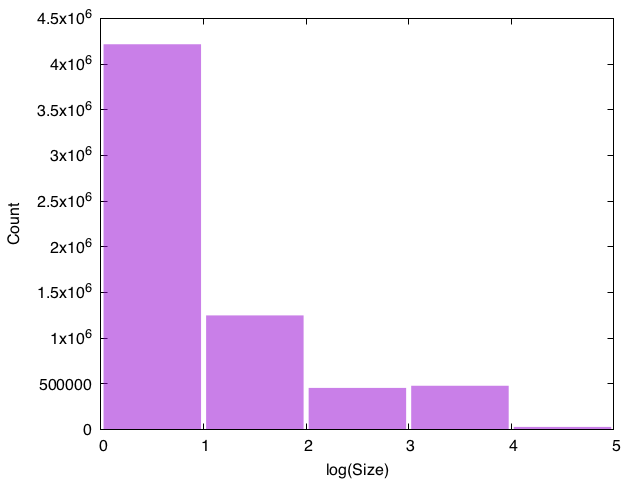
\includegraphics[width=0.6\textwidth]{figures/messageSizeHistogramNekbone}
\caption{Logarithmic histogram of message sizes sent by Nekbone application}
\label{fig:nekboneSizeHistogram}
\end{figure}

\subsection{Congestion Delay Histogram}
\label{subsec:congestionDelayHistogram}

A more involved example looks at congestion delays in the application.
We want to generate a histogram showing the aggregate delay (relative to zero-congestion baseline) that a packet experiences
going from source to destination.
By default, packets do not carry fields for measuring congestion. 
Thus, the packet allocator must be changed.
The NIC parameters now become:

\begin{ViFile}
nic {
 packet_allocator = delay_stats
 ejection {
  stats = delay_histogram
  delay_histogram {
   fileroot = delay
   bin_size = 0.5us
  }
 }
}
\end{ViFile}
The delay histogram goes in the ejection namespace since we want to measure packet congestion after it leaves the network.
The histogram is not logarithmic and we want to bin files in units of 0.5$\mu$s.
After running, two files will be generated: a gnuplot script\inlineshell{delay.p} and a corresponding data file \inlineshell{delay.dat}.
After running
\begin{ShellCmd}
shell>gnuplot delay.p 
\end{ShellCmd}
a PNG file \inlineshell{delay.png} is generated.
The generated histogram is shown in Figure \ref{fig:nekboneDelayHistogram}. 
Delays, when occurring in this case, are usually on the order of a few $\mu$s.

\begin{figure}
\centering
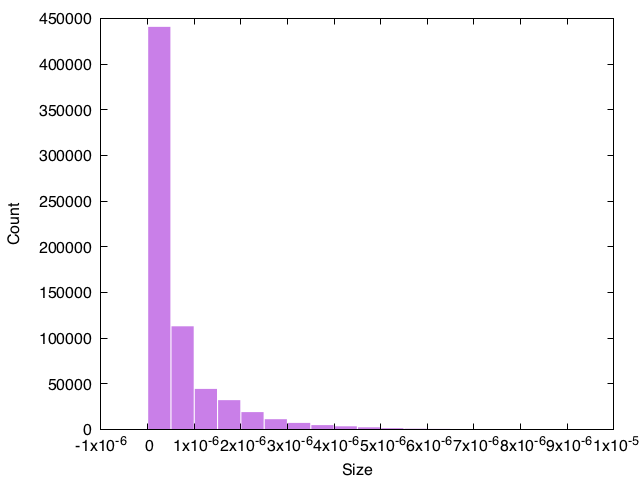
\includegraphics[width=0.6\textwidth]{figures/delayHistogramNekbone}
\caption{Histogram of message sizes sent by Nekbone application}
\label{fig:nekboneDelayHistogram}
\end{figure}

A few more things are actually required to complete the input file.
The input file above only tells the NIC to create a histogram.
We still have to tell the crossbars and buffers on the network to accumulate the delays on the packet.
Otherwise the NIC will just see a zero delay.
The following extra parameters are required:

\begin{ViFile}
switch {
 xbar {
   stats = congestion_delay
 }
 output_buffer {
  stats = congestion_delay
 }
}
\end{ViFile}

\subsection{Congestion Spyplot and Multi-stats}
\label{subsec:congestionSpyplot}

Another way to look for congestion is to create a spyplot.
Each row/column is a source/destination pair.
In contrast to previous spyplots that show the amount of traffic,
a congestion spyplot shows the amount of network congestion experienced sending between two points.
Most of the same parameters from the delay histogram are required.
However, we now want to collect both a spyplot and the histogram.

\begin{ViFile}
nic {
 packet_allocator = delay_stats
 ejection {
  stats = multi
  callbacks = congestion_spyplot delay_histogram
  congestion_spyplot {
   fileroot = spyplot
   type = png
   normalization = 100000
  }
  delay_histogram {
   fileroot = delay
   bin_size = 0.5us
  }
 }
}
\end{ViFile}

We set the stats collector to \inlinefile{multi}.
We then supply the list of desired stats to the \inlinefile{callbacks} parameter.
Zooming into the Nekbone example, we can see congestion hotspots.
For the most part, very little congestion appears in Figure \ref{fig:nekboneCongestionSpyplot}.
However (at least for the Torus topology used here),
there are a few off-diagonal regions that show some congestion.

\begin{figure}
\centering
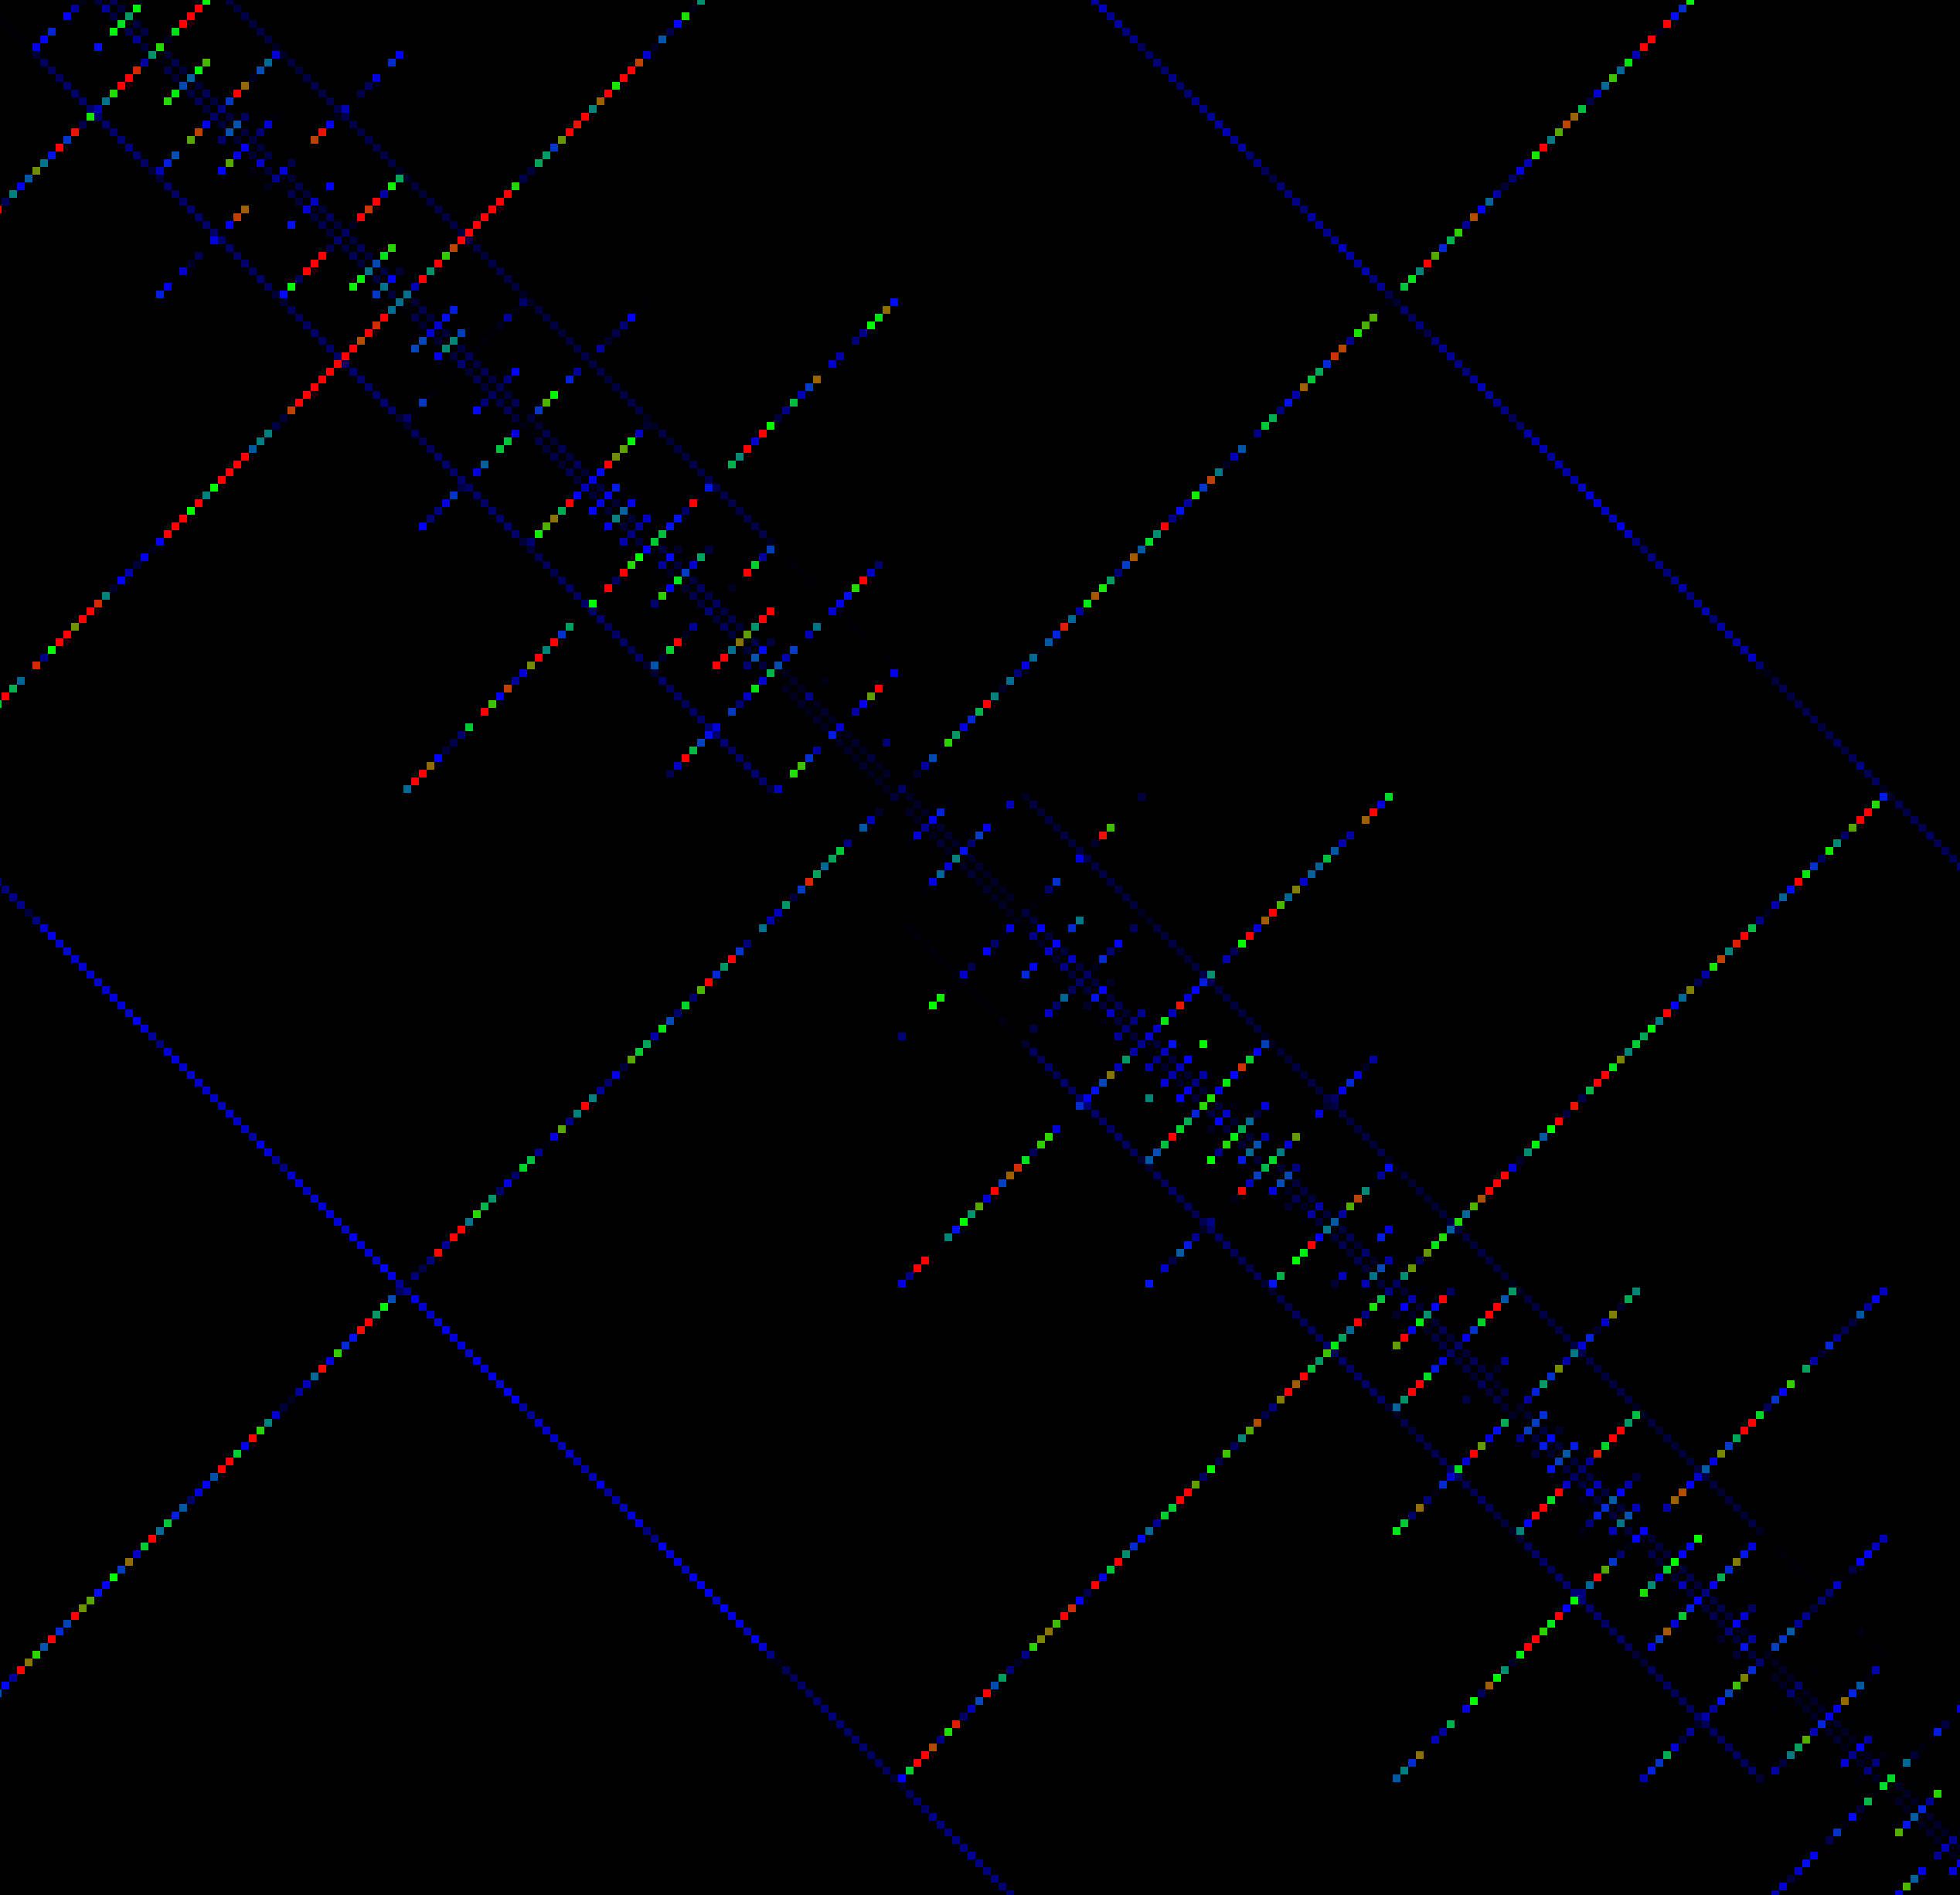
\includegraphics[width=0.6\textwidth]{figures/congestionSpyplotNekbone}
\caption{Spyplot showing congestion hotspots for certain source/destination pairs for Nekbone.}
\label{fig:nekboneCongestionSpyplot}
\end{figure}



